\newpage
%%%---> Original version
%\pgfdeclarehorizontalshading{myshadingA}
%{1cm}{rgb(0cm)=(1,0,0); color(2cm)=(green); color(4cm)=(blue)}
%\pgfuseshading{myshadingA}

%%%--> it's works
%\begin{textblock}{65}(-1,0)
%\pgfdeclarehorizontalshading{myshadingA}
%{2cm}{rgb(0cm)=(1,0,0); color(18.5cm)=(green); color(37cm)=(blue)}
%\pgfuseshading{myshadingA}
%\end{textblock}
%\mbox{}

\begin{textblock}{65}(-1,0)
\pgfdeclarehorizontalshading{myshadingA}
{27.1cm}{rgb(0cm)=(1,0,0); color(18.5cm)=(green); color(37cm)=(blue)}
\pgfuseshading{myshadingA}
\end{textblock}
\mbox{}

\newpage

\pgfdeclareverticalshading{myshadingC}
{4cm}{rgb(0cm)=(1,0,0); rgb(1.5cm)=(0,1,0); rgb(2cm)=(0,0,1)}
\pgfuseshading{myshadingC}

\pgfdeclareradialshading{sphere}{\pgfpoint{0.5cm}{0.5cm}}%
{rgb(0cm)=(0.9,0,0);
rgb(0.7cm)=(0.7,0,0);
rgb(1cm)=(0.5,0,0);
rgb(1.05cm)=(1,1,1)}
\pgfuseshading{sphere}


\pgfdeclarefunctionalshading[mycol]{sweep}{\pgfpoint{-1cm}{-1cm}}
{\pgfpoint{1cm}{1cm}}{\pgfshadecolortorgb{mycol}{\myrgb}}{
2 copy % whirl
% Calculate "safe" atan of position
2 copy abs exch abs add 0.0001 ge { atan } { pop } ifelse
3 1 roll
dup mul exch
dup mul add sqrt
30 mul
add
sin
1 add 2 div
dup
\myrgb % push mycol
5 4 roll % multiply all components by calculated value
mul
3 1 roll
3 index
mul
3 1 roll
4 3 roll
mul
3 1 roll
}
\colorlet{mycol}{white}%
\pgfuseshading{sweep}%
\colorlet{mycol}{red}%
\pgfuseshading{sweep}

% don't work
%\mycol=1.0 0.5 0.0 \mycolred=1.0 \mycolgreen=0.5 \mycolblue=0.0
%\pgfshadecolortorgb{orange}{\mycol}
%|\mycol|=\mycol |\mycolred|=\mycolred |\mycolgreen|=\mycolgreen |\mycolblue|=\mycolblue 
%
\pgfdeclarefunctionalshading[col1,col2,col3,col4]{bilinear interpolation}
{\pgfpointorigin}{\pgfpoint{100bp}{100bp}}
{
\pgfshadecolortorgb{col1}{\first}\pgfshadecolortorgb{col2}{\second}
\pgfshadecolortorgb{col3}{\third}\pgfshadecolortorgb{col4}{\fourth}
}{
100 div exch 100 div 2 copy % Calculate y/100 x/100.
neg 1 add exch neg 1 add % Calculate 1-y/100 1-x/100.
3 1 roll 2 copy exch 5 2 roll 6 copy 6 copy % Set up stack.
\firstred mul exch \secondred mul add mul % Process red component.
4 1 roll
\thirdred mul exch \fourthred mul add mul
add
13 1 roll
\firstgreen mul exch \secondgreen mul add mul % Process green component.
4 1 roll
\thirdgreen mul exch \fourthgreen mul add mul
add
7 1 roll
\firstblue mul exch \secondblue mul add mul % Process blue component.
4 1 roll
\thirdblue mul exch \fourthblue mul add mul
add
}
\colorlet{col1}{blue}
\colorlet{col2}{yellow}
\colorlet{col3}{red}
\colorlet{col4}{green}
%\pgfuseshading{bilinear interpolation}


\pgfdeclarefunctionalshading{twospots}
{\pgfpointorigin}{\pgfpoint{4cm}{4cm}}{}{
% Save coordinates for later
2 copy
% Compute distance from (40bp,45bp), with x doubled
45 sub dup mul exch
40 sub dup mul 0.5 mul add sqrt
% expontial decay
dup mul neg 1.0005 exch exp 1.0 exch sub
% Compute distance form (70bp,70bp) from stored coordiante, scaled
3 1 roll
70 sub dup mul .5 mul exch
70 sub dup mul add sqrt
% Decay
dup mul neg 1.002 exch exp 1.0 exch sub
% red component
1.0 3 1 roll
}
\pgfuseshading{twospots}


\newpage

\begin{pgfpicture}
	\pgfdeclareverticalshading{myshadingD}
	{20pt}{color(0pt)=(red); color(20pt)=(blue)}
	\pgftext[at=\pgfpoint{1cm}{0cm}] {\pgfuseshading{myshadingD}}
	\pgftext[at=\pgfpoint{2cm}{0.5cm}]{\pgfuseshading{myshadingD}}
\end{pgfpicture}

\pgfdeclareverticalshading{myshadingE}{100bp}
{color(0bp)=(red); color(25bp)=(green); color(75bp)=(blue);
color(100bp)=(black)}
\pgfuseshading{myshadingE}
\hskip 1cm
\begin{pgfpicture}
	\pgfpathrectangle{\pgfpointorigin}{\pgfpoint{2cm}{1cm}}
	\pgfshadepath{myshadingE}{0}
	\pgfusepath{stroke}
	\pgfpathrectangle{\pgfpoint{3cm}{0cm}}{\pgfpoint{1cm}{2cm}}
	\pgfshadepath{myshadingE}{0}
	\pgfusepath{stroke}
	\pgfpathrectangle{\pgfpoint{5cm}{0cm}}{\pgfpoint{2cm}{2cm}}
	\pgfshadepath{myshadingE}{45}
	\pgfusepath{stroke}
	\pgfpathcircle{\pgfpoint{9cm}{1cm}}{1cm}
	\pgfshadepath{myshadingE}{45}
	\pgfusepath{stroke}
\end{pgfpicture}


\newpage

\pgfdeclareverticalshading{myshadingF}{100bp}
{color(0bp)=(red); color(25bp)=(green); color(75bp)=(blue);
color(100bp)=(black)}
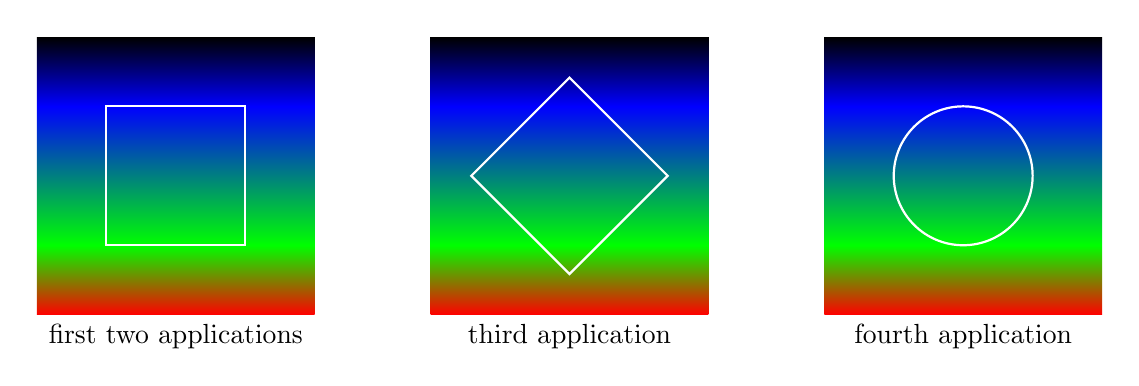
\begin{tikzpicture}
	\draw (50bp,50bp) node {\pgfuseshading{myshadingF}};
	\draw[white,thick] (25bp,25bp) rectangle (75bp,75bp);
	\draw (50bp,0bp) node[below] {first two applications};
	\begin{scope}[xshift=5cm]
		\draw (50bp,50bp) node{\pgfuseshading{myshadingF}};
		\draw[rotate around={45:(50bp,50bp)},white,thick] (25bp,25bp)
		rectangle (75bp,75bp);
		\draw (50bp,0bp) node[below] {third application};
	\end{scope}
	\begin{scope}[xshift=10cm]
		\draw (50bp,50bp) node{\pgfuseshading{myshadingF}};
		\draw[white,thick] (50bp,50bp) circle (25bp);
		\draw (50bp,0bp) node[below] {fourth application};
	\end{scope}
\end{tikzpicture}

\newpage

\pgfdeclareradialshading{ballshading}{\pgfpoint{-10bp}{10bp}}
{color(0bp)=(red!15!white); color(9bp)=(red!75!white);
color(18bp)=(red!70!black); color(25bp)=(red!50!black);
color(50bp)=(black)}
\pgfuseshading{ballshading}
\hskip 1cm
\begin{pgfpicture}
	\pgfpathrectangle{\pgfpointorigin}{\pgfpoint{1cm}{1cm}}
	\pgfshadepath{ballshading}{0}
	\pgfusepath{}
	\pgfpathcircle{\pgfpoint{3cm}{0cm}}{1cm}
	\pgfshadepath{ballshading}{0}
	\pgfusepath{}
	\pgfpathcircle{\pgfpoint{6cm}{0cm}}{1cm}
	\pgfshadepath{ballshading}{45}
	\pgfusepath{}
\end{pgfpicture}

\newpage
\vglue 25pt

\pgfdeclareverticalshading{myshadingG}{100bp}
{color(0bp)=(red); color(25bp)=(green); color(75bp)=(blue);
color(100bp)=(black)}
\begin{pgfpicture}
	\pgfpathrectangle{\pgfpointorigin}{\pgfpoint{2cm}{1cm}}
	\pgfshadepath{myshadingG}{0}
	\pgfusepath{stroke}
	\pgfpathrectangle{\pgfpoint{3cm}{0cm}}{\pgfpoint{2cm}{1cm}}
	\pgfshadepath{myshadingG}{90}
	\pgfusepath{stroke}
	\pgfpathrectangle{\pgfpoint{6cm}{0cm}}{\pgfpoint{2cm}{1cm}}
	\pgfshadepath{myshadingG}{45}
	\pgfusepath{stroke}
\end{pgfpicture}

\newpage
\vglue 25pt

\pgfdeclareverticalshading{rainbow}{100bp}
{color(0bp)=(red); color(25bp)=(red); color(35bp)=(yellow);
color(45bp)=(green); color(55bp)=(cyan); color(65bp)=(blue);
color(75bp)=(violet); color(100bp)=(violet)}
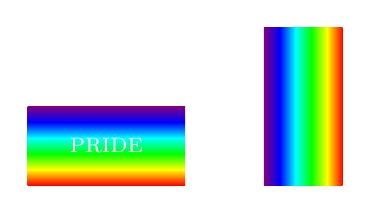
\begin{tikzpicture}[shading=rainbow]
	\shade (0,0) rectangle node[white] {\textsc{pride}} (2,1);
	\shade[shading angle=90] (3,0) rectangle +(1,2);
\end{tikzpicture}

\newpage
\vglue 25pt

\begin{pgfpicture}
	\pgfsetlinewidth{5mm}
	\color{red}
	\pgfpathcircle{\pgfpoint{0cm}{0cm}}{10mm} \pgfusepath{stroke}
	\color{black}
	\pgfsetstrokeopacity{0.5}
	\pgfpathcircle{\pgfpoint{1cm}{0cm}}{10mm} \pgfusepath{stroke}
\end{pgfpicture}

\newpage
\vglue 25pt

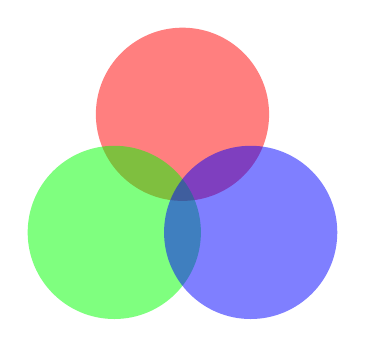
\begin{tikzpicture}
	\pgfsetfillopacity{0.5}
	\fill[red] (90:1cm) circle (11mm);
	\fill[green] (210:1cm) circle (11mm);
	\fill[blue] (-30:1cm) circle (11mm);
\end{tikzpicture}

\newpage
\vglue 25pt

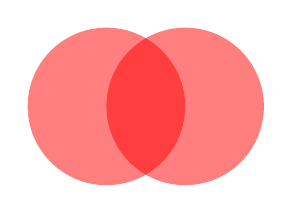
\begin{tikzpicture}
	\pgfsetfillopacity{0.5}
	\fill[red] (0,0) circle (1);
	\fill[red] (1,0) circle (1);
\end{tikzpicture}

\newpage
\vglue 25pt
\pgfdeclarefading{fading1}{\color{white}Ti\emph{k}Z}

\begin{tikzpicture}
	\fill [black!20] (0,0) rectangle (2,2);
	\fill [black!30] (0,0) arc (180:0:1);
	\pgfsetfading{fading1}{\pgftransformshift{\pgfpoint{1cm}{1cm}}}
	\fill [red] (0,0) rectangle (2,2);
\end{tikzpicture}

\newpage
\vglue 25pt
\pgfdeclarefading{fading2}
{\tikz \shade[left color=pgftransparent!0,
right color=pgftransparent!100] (0,0) rectangle (2,2);}

\begin{tikzpicture}
	\fill [black!20] (0,0) rectangle (2,2);
	\fill [black!30] (0,0) arc (180:0:1);
	\pgfsetfading{fading2}{\pgftransformshift{\pgfpoint{1cm}{1cm}}}
	\fill [red] (0,0) rectangle (2,2);
\end{tikzpicture}

\newpage
\vglue 25pt
\pgfdeclareradialshading{myshading}{\pgfpointorigin}
{
color(0mm)=(pgftransparent!0);
color(5mm)=(pgftransparent!0);
color(8mm)=(pgftransparent!100);
color(15mm)=(pgftransparent!100)
}
\pgfdeclarefading{fading3}{\pgfuseshading{myshading}}

\begin{tikzpicture}
	\fill [black!20] (0,0) rectangle (2,2);
	\fill [black!30] (0,0) arc (180:0:1);
	\pgfsetfading{fading3}{\pgftransformshift{\pgfpoint{1cm}{1cm}}}
	\fill [red] (0,0) rectangle (2,2);
\end{tikzpicture}

\newpage
\vglue 25pt
\pgfdeclarefading{fading2}
{\tikz \shade[left color=pgftransparent!0,
right color=pgftransparent!100] (0,0) rectangle (2,2);}

\begin{tikzpicture}
	\fill [black!20] (0,0) rectangle (2,2);
	\fill [black!30] (0,0) arc (180:0:1);
	\pgfsetfading{fading2}{}
	\fill [red] (0,0) rectangle (2,2);
\end{tikzpicture}

\newpage
\vglue 25pt

\begin{tikzpicture}
	\fill [black!20] (0,0) rectangle (2,2);
	\fill [black!30] (0,0) arc (180:0:1);
	\pgfsetfading{fading2}{\pgftransformshift{\pgfpoint{1cm}{1cm}}
	\pgftransformrotate{20}}
	\fill [red] (0,0) rectangle (2,2);
\end{tikzpicture}

\newpage
\vglue 25pt
\pgfdeclarehorizontalshading{shading}{100bp}
{ color(0pt)=(transparent!0); color(25bp)=(transparent!0);
color(75bp)=(transparent!100); color(100bp)=(transparent!100)}
\pgfdeclarefading{fading}{\pgfuseshading{shading}}

\begin{tikzpicture}
	\fill [black!20] (0,0) rectangle (2,2);
	\fill [black!30] (0,0) arc (180:0:1);
	\pgfpathrectangle{\pgfpointorigin}{\pgfpoint{2cm}{1cm}}
	\pgfsetfadingforcurrentpath{fading}{}
	\pgfusepath{discard}
	\fill [red] (0,0) rectangle (2,1);
	\pgfpathrectangle{\pgfpoint{0cm}{1cm}}{\pgfpoint{2cm}{1cm}}
	\pgfsetfadingforcurrentpath{fading}{\pgftransformrotate{90}}
	\pgfusepath{discard}
	\fill [red] (0,1) rectangle (2,2);
\end{tikzpicture}

\newpage
\vglue 25pt
\begin{tikzpicture}
	\draw [help lines] (0,0) grid (2,2);
	% Stuff outside the picture, but still in a transparency group.
	\node [left,overlay] at (0,1) {
	\begin{tikzpicture}
		\pgfsetfillopacity{0.5}
		\pgftransparencygroup
		\node at (2,0) [forbidden sign,line width=2ex,draw=red,fill=white]
		{Smoking};
		\endpgftransparencygroup
	\end{tikzpicture}
	};
\end{tikzpicture}

\newpage
\vglue 25pt
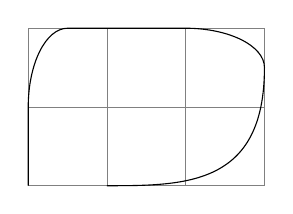
\begin{tikzpicture}
	\draw[help lines] (0,0) grid (3,2);
	\pgfsetcornersarced{\pgfpoint{10mm}{5mm}}
	% 10mm entering,
	% 5mm leaving.
	\pgfpathmoveto{\pgfpointorigin}
	\pgfpathlineto{\pgfpoint{0cm}{2cm}}
	\pgfpathlineto{\pgfpoint{3cm}{2cm}}
	\pgfpathcurveto
	{\pgfpoint{3cm}{0cm}}
	{\pgfpoint{2cm}{0cm}}
	{\pgfpoint{1cm}{0cm}}
	\pgfusepath{stroke}
\end{tikzpicture}

\newpage
\vglue 25pt
\begin{pgfpicture}
	% Half-parabola going ``up and right''
	\pgfpathmoveto{\pgfpointorigin}
	\pgfpathparabola{\pgfpointorigin}{\pgfpoint{2cm}{4cm}}
	\color{red}
	\pgfusepath{stroke}
	% Half-parabola going ``down and right''
	\pgfpathmoveto{\pgfpointorigin}
	\pgfpathparabola{\pgfpoint{-2cm}{4cm}}{\pgfpointorigin}
	\color{blue}
	\pgfusepath{stroke}
	% Full parabola
	\pgfpathmoveto{\pgfpoint{-2cm}{2cm}}
	\pgfpathparabola{\pgfpoint{1cm}{-1cm}}{\pgfpoint{2cm}{4cm}}
	\color{orange}
	\pgfusepath{stroke}
\end{pgfpicture}

\newpage
\vglue 25pt
\begin{pgfpicture}
	\pgfsetlinewidth{0.8pt}
	\pgfpathgrid[step={\pgfpoint{1cm}{1cm}}]
	{\pgfpoint{-3mm}{-3mm}}{\pgfpoint{33mm}{23mm}}
	\pgfusepath{stroke}
	\pgfsetlinewidth{0.4pt}
	\pgfpathgrid[stepx=1mm,stepy=1mm]
	{\pgfpoint{-1.5mm}{-1.5mm}}{\pgfpoint{31.5mm}{21.5mm}}
	\pgfusepath{stroke}
\end{pgfpicture}

\newpage
\vglue 25pt
\begin{pgfpicture}
	\pgftransformrotate{10}
	\pgfpathgrid[stepx=1mm,stepy=2mm]{\pgfpoint{0mm}{0mm}}{\pgfpoint{30mm}{30mm}}
	\pgfusepath{stroke}
\end{pgfpicture}

\newpage
\vglue 25pt
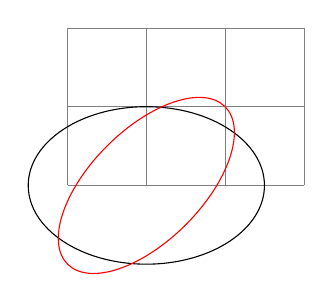
\begin{tikzpicture}
	\draw[help lines] (0,0) grid (3,2);
	\pgfpathellipse{\pgfpoint{1cm}{0cm}}
	{\pgfpoint{1.5cm}{0cm}}
	{\pgfpoint{0cm}{1cm}}
	\pgfusepath{draw}
	\color{red}
	\pgfpathellipse{\pgfpoint{1cm}{0cm}}
	{\pgfpoint{1cm}{1cm}}
	{\pgfpoint{-0.5cm}{0.5cm}}
	\pgfusepath{draw}
\end{tikzpicture}

\newpage
\vglue 25pt
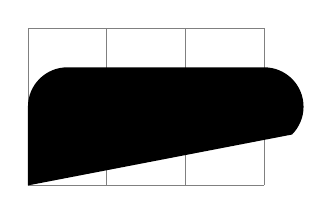
\begin{tikzpicture}
	\draw[help lines] (0,0) grid (3,2);
	\pgfpathmoveto{\pgfpointorigin}
	\pgfpathlineto{\pgfpoint{0cm}{1cm}}
	\pgfpatharc{180}{90}{.5cm}
	\pgfpathlineto{\pgfpoint{3cm}{1.5cm}}
	\pgfpatharc{90}{-45}{.5cm}
	\pgfusepath{fill}
\end{tikzpicture}
%%- page 576
\newpage
\vglue 25pt
\begin{pgfpicture}
	\pgfpathmoveto{\pgfpointorigin}
	\pgfpathcurveto
	{\pgfpoint{1cm}{1cm}}{\pgfpoint{2cm}{1cm}}{\pgfpoint{3cm}{0cm}}
	\pgfsetfillcolor{red}
	\pgfusepath{fill,stroke}
\end{pgfpicture}

\newpage
\vglue 25pt
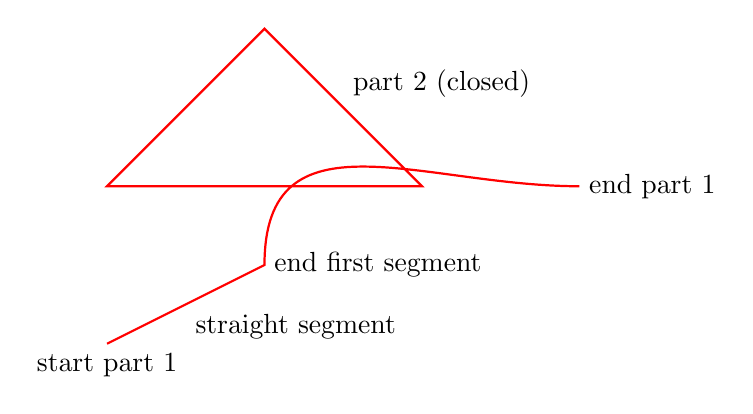
\begin{tikzpicture}[scale=2]
	\draw[thick,red]
	(0,0) coordinate (a)
	-- coordinate (ab) (1,.5) coordinate (b)
	.. coordinate (bc) controls +(up:1cm) and +(left:1cm) .. (3,1)
	coordinate (c)
	(0,1) -- (2,1) -- coordinate (x) (1,2) -- cycle;
	\draw (a) node[below] {start part 1}
	(ab) node[below right] {straight segment}
	(b) node[right] {end first segment}
	(c) node[right] {end part 1}
	(x) node[above right] {part 2 (closed)};
\end{tikzpicture}

\newpage
\vglue 25pt
\begin{pgfpicture}
	\foreach \x in {1,...,50}{
	\pgfmathrandominteger{\a}{1}{50}
	\pgfmathrandominteger{\b}{1}{50}
	\pgfpathcircle{\pgfpoint{+\a pt}{+\b pt}}{+2pt}
	\color{blue!40!white}
	\pgfsetstrokecolor{blue!80!black}
	\pgfusepath{stroke, fill}
	}
\end{pgfpicture}

\newpage
\vglue 25pt
\begin{pgfpicture}
	\pgfmathdeclarerandomlist{color}{{red}{blue}{green}{yellow}{white}}
	\foreach \a in {1,...,50}{
	\pgfmathrandominteger{\x}{1}{85}
	\pgfmathrandominteger{\y}{1}{85}
	\pgfmathrandominteger{\r}{5}{10}
	\pgfmathrandomitem{\c}{color}
	\pgfpathcircle{\pgfpoint{+\x pt}{+\y pt}}{+\r pt}
	\color{\c!40!white}
	\pgfsetstrokecolor{\c!80!black}
	\pgfusepath{stroke, fill}
	}
\end{pgfpicture}

%%%%--->

\newpage

\pgfdeclarelayer{background layer}
\pgfdeclarelayer{foreground layer}
\pgfsetlayers{background layer,main,foreground layer}
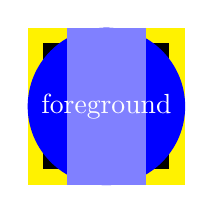
\begin{tikzpicture}
	% On main layer:
	\fill[blue] (0,0) circle (1cm);
	\begin{pgfonlayer}{background layer}
		\fill[yellow] (-1,-1) rectangle (1,1);
	\end{pgfonlayer}
	\begin{pgfonlayer}{foreground layer}
		\node[white] {foreground};
	\end{pgfonlayer}
	\begin{pgfonlayer}{background layer}
		\fill[black] (-.8,-.8) rectangle (.8,.8);
	\end{pgfonlayer}
	% On main layer again:
	\fill[blue!50] (-.5,-1) rectangle (.5,1);
\end{tikzpicture}

\begin{center}

\begin{tikzpicture}[decoration={footprints,foot length=20pt}]
	\fill [decorate] (0,0) -- (3,0);
\end{tikzpicture}

\vglue 15pt

\begin{tikzpicture}[decoration={footprints,stride length=50pt}]
	\fill [decorate] (0,0) -- (3,0);
\end{tikzpicture}

\vglue 15pt

\begin{tikzpicture}[decoration={footprints,foot sep=10pt}]
	\fill [decorate] (0,0) -- (3,0);
\end{tikzpicture}

\vglue 15pt

\begin{tikzpicture}[decoration={footprints,foot angle=60}]
	\fill [decorate] (0,0) -- (3,0);
\end{tikzpicture}

\vglue 15pt

\begin{tikzpicture}
	\path[mindmap,concept color=black,text=white]
	node[concept] {Computer Science}
	[clockwise from=0]
	child[concept color=green!50!black] {
	node[concept] {practical}
	[clockwise from=90]
	child { node[concept] {algorithms} }
	child { node[concept] {data structures} }
	child { node[concept] {pro\-gramming languages} }
	child { node[concept] {software engineer\-ing} }
	}
	child[concept color=blue] {
	node[concept] {applied}
	[clockwise from=-30]
	child { node[concept] {databases} }
	child { node[concept] {WWW} }
	}
	child[concept color=red] { node[concept] {technical} }
	child[concept color=orange] { node[concept] {theoretical} };
\end{tikzpicture}

\begin{minipage}{3.5cm}\raggedright
	\color{red}Red text,%
	\begin{colormixin}{25!white}
		washed-out red text,
		\color{blue} washed-out blue text,
		\begin{colormixin}{25!black}
			dark washed-out blue text,
			\color{green} dark washed-out green text,%
		\end{colormixin}
		back to washed-out blue text,%
	\end{colormixin}
	and back to red.
\end{minipage}%

\newpage
\vglue 15pt

\pgfmathsetseed{1}
\foreach \col in {black,red,green,blue}
{
\begin{tikzpicture}[x=10pt,y=10pt,ultra thick,baseline,line cap=round]
	\coordinate (current point) at (0,0);
	\coordinate (old velocity) at (0,0);
	\coordinate (new velocity) at (rand,rand);
	\foreach \i in {0,1,...,100}
	{
	\draw[\col!\i] (current point)
	.. controls ++([scale=-1]old velocity) and
	++(new velocity) .. ++(rand,rand)
	coordinate (current point);
	\coordinate (old velocity) at (new velocity);
	\coordinate (new velocity) at (rand,rand);
	}
\end{tikzpicture}
}

\begin{tikzpicture}
	\node[chamfered rectangle, white, fill=red, double=red, draw, very
	thick]
	{\bf STOP!};
\end{tikzpicture}

\newpage
\begin{tikzpicture}
	\foreach \i in {1,...,4}
	\node[starburst,drop shadow,fill=white,draw] at (0,\i) {Burst \i};
\end{tikzpicture}

\begin{tikzpicture}
	\node [forbidden sign,line width=1ex,draw=red,fill=white] {Smoking};
\end{tikzpicture}

\begin{tikzpicture}[aspect=1, every node/.style={cloud, cloud puffs=11,
	draw}]
	\node [fill=gray!20] {rain};
	\node [cloud ignores aspect, fill=white] at (1.5,0) {snow};
\end{tikzpicture}

\newpage
\begin{tikzpicture}
	\node[starburst, fill=yellow, draw=red, line width=2pt] {\bf BANG!};
\end{tikzpicture}

\begin{tikzpicture}
	\draw[help lines] grid(3,2);
	\node[starburst, draw, minimum width=3cm, minimum height=2cm]
	at (1.5, 1) {\bf BOOM!};
\end{tikzpicture}

\newpage
\begin{tikzpicture}
	[every node/.style={signal, draw, text=white, signal to=nowhere}]
	\node[fill=green!65!black, signal to=east] at (0,1) {To East};
	\node[fill=red!65!black, signal from=east] at (0,0) {From East};
\end{tikzpicture}

\begin{tikzpicture}
	\node[cloud callout, cloud puffs=15, aspect=2.5, cloud puff arc=120,
	shading=ball,text=white] {\bf Imagine...};
\end{tikzpicture}

\begin{tikzpicture}
	\draw[help lines] (0,0) grid (3,2);
	\node [cross out,draw=red] at (1.5,1) {cross out};
\end{tikzpicture}
\end{center}

---> new shapes page 622 !

\newpage
\pgfrememberpicturepositiononpagetrue
\begin{pgfpicture}
	\pgfusepath{use as bounding box}
	\pgftransformshift{\pgfpointanchor{current page}{south west}}
	\pgftransformshift{\pgfpoint{1cm}{1cm}}
	\pgftext[left,base]{
	\textcolor{red}{
	Text absolutely positioned in
	the lower left corner.}
	}
\end{pgfpicture}

\newpage
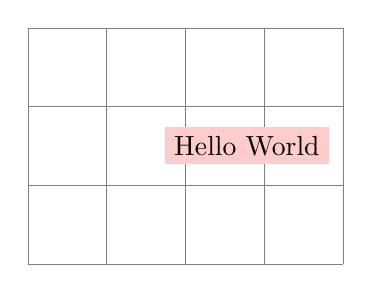
\begin{tikzpicture}
	\draw[help lines] (0,0) grid (4,3);
	{
	\color{red!20}
	\pgftransformrotate{10}
	\pgftransformshift{\pgfpoint{3cm}{1cm}}
	\pgftransformresetnontranslations
	\pgfnode{rectangle}{center}
	{\color{black}Hello World}{hellonode}{\pgfusepath{fill}}
	}
\end{tikzpicture}


\newpage
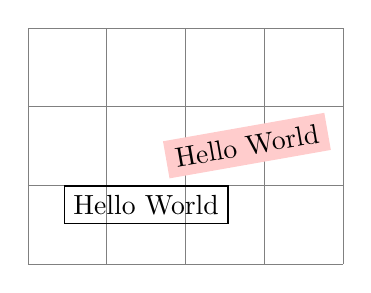
\begin{tikzpicture}
	\draw[help lines] (0,0) grid (4,3);
	{
	\pgftransformshift{\pgfpoint{1.5cm}{1cm}}
	\pgfnode{rectangle}{north}{Hello World}{hellonode}{\pgfusepath{stroke}}
	}
	{
	\color{red!20}
	\pgftransformrotate{10}
	\pgftransformshift{\pgfpoint{3cm}{1cm}}
	\pgfnode{rectangle}{center}
	{\color{black}Hello World}{hellonode}{\pgfusepath{fill}}
	}
\end{tikzpicture}

\newpage
\vglue 25pt

\tikz \path decorate [decoration={text along path,
text={Some text along a path}}]
{ (0,2) .. controls (2,2) and (1,0) .. (3,0) };

\newpage
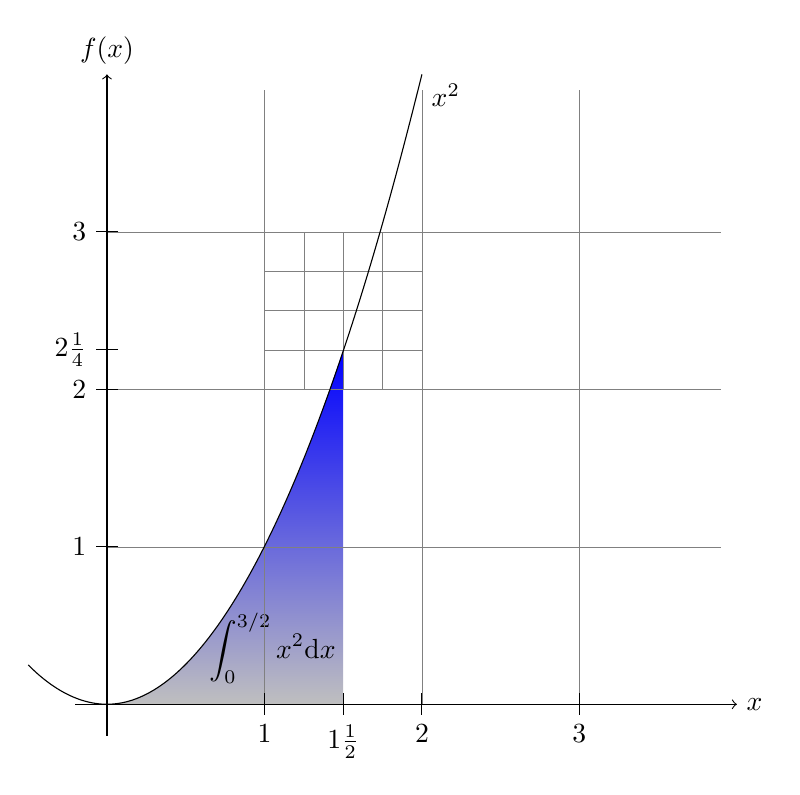
\begin{tikzpicture}[scale=2]
	\shade[top color=blue,bottom color=gray!50] (0,0) parabola (1.5,2.25)
	|- (0,0);
	\draw (1.05cm,2pt) node[above] {$\displaystyle\int_0^{3/2}
	x^2\mathrm{d}x$};
	\draw[help lines] (0,0) grid (3.9,3.9)
	[step=0.25cm] (1,2) grid +(1,1);
	\draw[->] (-0.2,0) -- (4,0) node[right] {$x$};
	\draw[->] (0,-0.2) -- (0,4) node[above] {$f(x)$};
	\foreach \x/\xtext in {1/1, 1.5/1\frac{1}{2}, 2/2, 3/3}
	\draw[shift={(\x,0)}] (0pt,2pt) -- (0pt,-2pt) node[below] {$\xtext$};
	\foreach \y/\ytext in {1/1, 2/2, 2.25/2\frac{1}{4}, 3/3}
	\draw[shift={(0,\y)}] (2pt,0pt) -- (-2pt,0pt) node[left] {$\ytext$};
	\draw (-.5,.25) parabola bend (0,0) (2,4) node[below right] {$x^2$};
\end{tikzpicture}

\newpage

\begin{tikzpicture}[remember picture]
	\node[ellipse callout, draw] (hallo) {Hallo!};
\end{tikzpicture}

\begin{tikzpicture}[remember picture, note/.style={rectangle callout,
	fill=#1}]
	\draw [help lines] grid(3,2);
	\node [note=red!50, callout relative pointer={(0,1)}] at (3,1)
	{Relative};
	\node [note=blue!50, callout absolute pointer={(0,1)}] at (1,0)
	{Absolute};
	\node [note=green!50, opacity=.5, overlay,
	callout absolute pointer={(hallo.south)}] at (1,2) {Outside};
\end{tikzpicture}


\begin{tikzpicture}
	\tikzset{callout/.style={ellipse callout, callout pointer arc=30,
	callout absolute pointer={#1}}}
	\draw (0,0) grid (3,2);
	\node[callout={(3,1.5)}, fill=red!50] at (0,1.5) {A};
	\node[callout={(3,.5)}, fill=green!50, callout pointer shorten=1cm]
	at (0,.5) {B};
\end{tikzpicture}

\newpage

\tikz \draw[top color=red] (0,0) rectangle (2,1);
\tikz \draw[top color=white,bottom color=black,middle color=red]
(0,0) rectangle (2,1);
\tikz \draw[inner color=red] (0,0) rectangle (2,1);
\tikz \draw[outer color=red,inner color=white]
(0,0) rectangle (2,1);

\newpage
\sffamily\scriptsize
\begin{tikzpicture}
	[transform shape,
	every calendar/.style=
	{
	at={(-8ex,4ex)},
	week list,
	month label above centered,
	month text=\bfseries\textcolor{red}{\%mt} \%y0,
	if={(Sunday) [black!50]}
	}]
	\tikzfoldingdodecahedron
	[
	folding line length=2.5cm,
	face 1={ \calendar [dates=\the\year-01-01 to \the\year-01-last];},
	face 2={ \calendar [dates=\the\year-02-01 to \the\year-02-last];},
	face 3={ \calendar [dates=\the\year-03-01 to \the\year-03-last];},
	face 4={ \calendar [dates=\the\year-04-01 to \the\year-04-last];},
	face 5={ \calendar [dates=\the\year-05-01 to \the\year-05-last];},
	face 6={ \calendar [dates=\the\year-06-01 to \the\year-06-last];},
	face 7={ \calendar [dates=\the\year-07-01 to \the\year-07-last];},
	face 8={ \calendar [dates=\the\year-08-01 to \the\year-08-last];},
	face 9={ \calendar [dates=\the\year-09-01 to \the\year-09-last];},
	face 10={\calendar [dates=\the\year-10-01 to \the\year-10-last];},
	face 11={\calendar [dates=\the\year-11-01 to \the\year-11-last];},
	face 12={\calendar [dates=\the\year-12-01 to \the\year-12-last];}
	];
\end{tikzpicture}

\newpage

\tikz[mindmap,concept color=blue!80]
\node [concept] {Root concept}
child[concept color=red,grow=30] {node[concept] {Child concept}}
child[concept color=orange,grow=0] {node[concept] {Child concept}};

\tikz
[root concept/.append style={concept color=blue!80},
level 1 concept/.append style={concept color=red!50},
mindmap]
\node [concept] {Root concept}
child[grow=30] {node[concept] {child}}
child[grow=0 ] {node[concept] {child}};

\tikz[mindmap,text=white,
root concept/.style={concept color=blue},
level 1 concept/.append style=
{every child/.style={concept color=blue!50}}]
\node [concept] {Root concept}
child[grow=30] {node[concept] {child}}
child[grow=0 ] {node[concept] {child}};

\begin{tikzpicture}
	[root concept/.append style={concept color=blue!20,minimum size=2cm},
	level 1 concept/.append style={sibling angle=45},
	mindmap]
	\node [concept] {Root concept}
	[clockwise from=45]
	child { node[concept] (c1) {child}}
	child { node[concept] (c2) {child}}
	child { node[concept] (c3) {child}};
	\begin{pgfonlayer}{background}
		\draw [concept connection] (c1) edge (c2)
		edge (c3)
		(c2) edge (c3);
	\end{pgfonlayer}
\end{tikzpicture}

\begin{tikzpicture}[outer sep=0pt]
	\node (n1) at (0,0) [circle,minimum size=2cm,fill,draw,thick,red] {};
	\node (n2) at (30:2.5) [circle,minimum size=1cm,fill,draw,thick,blue]
	{};
	\path (n1) to[circle connection bar switch color=from (red) to (blue)]
	(n2);
\end{tikzpicture}

\newpage

\begin{tikzpicture}
	\draw [help lines] grid (3,2);
	\path [decorate,decoration={text along path,
	text={a |\large|big |+\bf\color{red}|red|| juicy apple.}}]
	(0,0) .. controls (0,2) and (3,0) .. (3,2);
\end{tikzpicture}

\newpage

%%%--->

\tikzfading[name=middle,
top color=transparent!50,
bottom color=transparent!50,
middle color=transparent!20]
\begin{tikzpicture}
	\node [circle,circular drop shadow,
	pattern=horizontal lines dark blue,
	path fading=south,
	minimum size=3.6cm] {};
	\pattern [path fading=north,
	pattern=horizontal lines dark gray]
	(0,0) circle (1.8cm);
	\pattern [path fading=middle,
	pattern=crosshatch dots light steel blue]
	(0,0) circle (1.8cm);
\end{tikzpicture}

\tikzfading[name=fade inside,
inner color=transparent!80,
outer color=transparent!30]
\begin{tikzpicture}
	% Checker board
	\fill [black!20] (0,0) rectangle (4,4);
	\path [pattern=checkerboard,pattern color=black!30] (0,0) rectangle
	(4,4);
	\shade [ball color=red] (3,3) circle (0.8);
	\shade [ball color=white,path fading=fade inside] (2,2) circle (1.8);
\end{tikzpicture}

\begin{tikzpicture}
	% Checker board
	\fill [black!20] (0,0) rectangle (4,4);
	\path [pattern=checkerboard,pattern color=black!30] (0,0) rectangle
	(4,4);
	\shade [ball color=blue,path fading=south] (2,2) circle (1.8);
\end{tikzpicture}

%\begin{tikzpicture}[path fading=fade down]
%	% Checker board
%	\fill [black!20] (0,0) rectangle (4,1.5);
%	\path [pattern=checkerboard,pattern color=black!30] (0,0) rectangle
%	(4,1.5);
%	\fill [red,path fading,fading transform={rotate=90}]
%	(1,0.75) ellipse (.75 and .5);
%	\fill [red,path fading,fading transform={rotate=30}]
%	(3,0.75) ellipse (.75 and .5);
%\end{tikzpicture}

\begin{tikzpicture}[path fading=south]
	% Checker board
	\fill [black!20] (0,0) rectangle (4,3);
	\pattern [pattern=checkerboard,pattern color=black!30]
	(0,0) rectangle (4,3);
	\fill [color=blue] (0.5,1.5) rectangle +(1,1);
	\fill [color=blue,path fading=north] (2.5,1.5) rectangle +(1,1);
	\fill [color=red,path fading] (1,0.75) ellipse (.75 and .5);
	\fill [color=red] (3,0.75) ellipse (.75 and .5);
\end{tikzpicture}

\tikzfading[name=fade out,
inner color=transparent!0,
outer color=transparent!100]
% Now we use the fading in another picture:
\begin{tikzpicture}
	% Background
	\fill [black!20] (-1.2,-1.2) rectangle (1.2,1.2);
	\path [pattern=checkerboard,pattern color=black!30]
	(-1.2,-1.2) rectangle (1.2,1.2);
	\fill [blue,path fading=fade out] (-1,-1) rectangle (1,1);
\end{tikzpicture}

\tikzfading[name=fade right,
left color=transparent!0,
right color=transparent!100]
% Now we use the fading in another picture:
\begin{tikzpicture}
	% Background
	\fill [black!20] (-1.2,-1.2) rectangle (1.2,1.2);
	\path [pattern=checkerboard,pattern color=black!30]
	(-1.2,-1.2) rectangle (1.2,1.2);
	\fill [red,path fading=fade right] (-1,-1) rectangle (1,1);
\end{tikzpicture}

\begin{tikzfadingfrompicture}[name=tikz]
	\node [text=transparent!20]
	{\fontfamily{ptm}\fontsize{45}{45}\bfseries\selectfont Ti\emph{k}Z};
\end{tikzfadingfrompicture}

% Now we use the fading in another picture:
\begin{tikzpicture}
	\fill [black!20] (-2,-1) rectangle (2,1);
	\pattern [pattern=checkerboard,pattern color=black!30]
	(-2,-1) rectangle (2,1);
	\shade[path fading=tikz,fit fading=false,
	left color=blue,right color=black]
	(-2,-1) rectangle (2,1);
\end{tikzpicture}

%%%--->
\begin{tikzfadingfrompicture}[name=fade right]
	\shade[left color=transparent!0,
	right color=transparent!100] (0,0) rectangle (2,2);
	\fill[transparent!50] (1,1) circle (0.7);
\end{tikzfadingfrompicture}
% Now we use the fading in another picture:
\begin{tikzpicture}
	% Background
	\fill [black!20] (-1.2,-1.2) rectangle (1.2,1.2);
	\pattern [pattern=checkerboard,pattern color=black!30]
	(-1.2,-1.2) rectangle (1.2,1.2);
	\fill [path fading=fade right,red] (-1,-1) rectangle (1,1);
\end{tikzpicture}

\begin{tikzpicture}
	[
	% Define an interesting style
	button/.style={
	% First preaction: Fuzzy shadow
	preaction={fill=black,path fading=circle with fuzzy edge 20 percent,
	opacity=.5,transform canvas={xshift=1mm,yshift=-1mm}},
	% Second preaction: Background pattern
	preaction={pattern=#1,
	path fading=circle with fuzzy edge 15 percent},
	% Third preaction: Make background shiny
	preaction={top color=white,
	bottom color=black!50,
	shading angle=45,
	path fading=circle with fuzzy edge 15 percent,
	opacity=0.2},
	% Fourth preaction: Make edge especially shiny
	preaction={path fading=fuzzy ring 15 percent,
	top color=black!5,
	bottom color=black!80,
	shading angle=45},
	inner sep=2ex
	},
	button/.default=horizontal lines light blue,
	circle
	]
	\draw [help lines] (0,0) grid (4,3);
	\node [button] at (2.2,1) {\Huge Big};
	\node [button=crosshatch dots light steel blue,
	text=white] at (1,1.5) {Small};
\end{tikzpicture}
